\documentclass[12pt, a4paper]{report}

\usepackage[style=authoryear,sorting=nyt]{biblatex}
\usepackage{glossaries}
\usepackage{graphicx}
\usepackage{hyperref}
\usepackage{setspace}
\usepackage{verbatim}


\addbibresource{references.bib}

\makeglossaries

\newacronym{icl}{ICL}{In-Context Learning}
\newacronym{llm}{LLM}{Lange Language Model}
\newacronym{npc}{NPC}{Non-Player Character}
\newacronym{moe}{MoE}{Mixture of Expert}
\newacronym{rag}{RAG}{Retrieval Augmented Generation}
\newacronym{tts}{TTS}{Text to Speech}

\singlespacing

\begin{document}
	\begin{titlepage}
		\centering
		
		\vspace*{1cm}
		
		\Huge\textbf{Evaluating Large Language Models for NPC Interaction in Games}
		
		\vfill
		
		\large
		
		\makebox[0pt][r]{Author} – \makebox[0pt][l]{Raiwin Lewis}
		
		\makebox[0pt][r]{Supervisor} – \makebox[0pt][l]{Frank Langbein}
		
		\makebox[0pt][r]{School} – \makebox[0pt][l]{Cardiff University}
		
		\vspace{1cm}
		
		May 7, 2026
		
		\vspace{2cm}
	\end{titlepage}
	
	\pagenumbering{roman}
	
	\chapter*{Abstract}
	\addcontentsline{toc}{chapter}{Abstract}
	Linear dialogue trees are a common occurrence in video games, providing an interesting story similar to a book or film, improving the experience through \gls{npc}s and cut-scenes. With games, we have the option of branching dialogue trees giving players choice within games, increasing replayability at the cost of developer work. What if games could generate dialogue in real-time allowing for unlimited possibilities. The primary aim is to evaluate whether \gls{llm}s could be used to generate dialogue by creating a murder mystery game with both scripted and \gls{llm} powered dialogue, improve \gls{llm} performance using techniques such as prompt-engineering to ground LLM knowledge to improve coherency and consistency and conduct a user evaluation compare a scripted and \gls{llm} powered dialogue to measure improvements in narrative consistency and player engagement. The model used is Qwen3.6-35b-a3b quantised to q4\_K\_M running externally to the client, using Pygame, written in python and participants asked to test both dialogue versions. The results suggesting that \gls{llm}s have the potential to enhance game experiences through \gls{npc}s but I was unable to reach where it would be considered viable.
	
	\chapter*{Acknowledgements}
	\addcontentsline{toc}{chapter}{Acknowledgements}
	I would like to thank my supervisor for the assistance throughout the process as well as all the participants for taking part.
	
	I would also like to acknowledge the use of AI. Gemma4 was used during the writing process of this report for structure and refinement. MiniMax M2.5 for suggestions regarding implementation of features in the murder mystery game but has been completely refactored before testing. MiniMax M2.5 was also used to fill out the story for the murder mystery game. All generated content was scrutinised and verified and as the author, take full responsibility for the final output.
	
	\tableofcontents
	\listoffigures
	\listoftables
	\printglossary[type=\acronymtype, title=List of Abbreviations]
	
	\newpage
	\pagenumbering{arabic}
	
	\chapter{Introduction}
	\section{Overview}
	\gls{npc}s play a significant role in games. \gls{npc}s immerse the player into the game world by interacting with the player, providing assistance and developing the story through one-on-one dialogue and cut-scenes. As modern games become increasingly complex, so has the dialogue system. One way developers are increasing complexity is through multiple paths leading to multiple endings allowing players to choose what path they want to take.
	
	With multiple paths, each path could have different dialogue and cut-scenes which we can sum up as dialogue trees. Increasing the number of paths or endings a player can take increases the complexity of the dialogue tree. This creates additional work for writers and developers, increasing exponentially as more paths are added which becomes harder to maintain and add to since it is easier for writers to forget a detail and create loop-holes in the story.
	
	Most games stick to a linear story similar to a book or film, but when developers build a game with multiple endings, its normal to find less than a dozen with interweaving paths in the story to keep the size of the dialogue tree from exploding too big.
	
	What if the dialogue could instead by generated in real-time as the player experiences the game. With \gls{llm}, we can dynamically generate text based on the story and any other relevant information to allow the story to have unlimited possibilities when it comes to dialogue.
	
	\section{Problem Statement}
	With scripted dialogue, answers are strict and may harm the replayability of games, especially ones that focus on story. One step up would be branching dialogue trees which allow players to choose their path within the game providing a unique experience. The replayability factor increases to as players may want to explore multiple paths within the game.
	
	LLMs would be a great step up in terms of progression in these dialogue systems allowing for dialogue to be dynamically generated providing a unique experience every time the game is played.
	
	However this has major issues. \gls{llm}s output can't be fully controlled, they may break character and go out of the defined scope it was given and hallucinate incorrect information. We tend to notice when something feels off quickly so this would break the experience for the player. \gls{llm}s also have the problem of the player "jailbreaking" or intentionally breaking it out of character to produced a result undesired by the developer. Another issue is that \gls{llm}s, due to the way they are built, have a lot of bias such as insinuating stereotypes makes adding personality to these \gls{npc}s more difficult.
	
	In certain games, \gls{llm}s would not be a good fit, such as games with a linear story where it is designed to guide the player down a set experience and would have no benefit with such a system as it would deviate from the games vision.
	
	One specific area in games which would also benefit from a \gls{llm} system is interaction between players and \gls{npc}s where the player is not directly talking to them. An example situation would be bumping into someone and getting a remark back, after a while you start to notice repeats in the scripted dialogue. With an \gls{llm} system, we could increase the variety of dialogue substantially, as well as the style of response, dynamically generated based on the type of \gls{npc}.

	It is worth noting that \gls{llm} only output text and would require a text-to-speech engine in order for audio to be played. This will need its own implementation as operating systems do not currently have customisable voices suitable for many \gls{npc}s a game would have and would need to be provided by the developer.
	
	\section{Aims and Objectives}
	The primary aim of this project is to explore whether using LLMs in games would enhance game experiences over the traditional scripted writing with optional branching trees.
	
	From the problem statement, we can define specific objectives as follows:
	
	\begin{enumerate}
		\item Develop a murder mystery game with both scripted and LLM powered dialogue system.
		\item Implement improvements using prompt-engineering or other techniques to ground LLM knowledge into the specified setting to improve coherency and consistency.
		\item Conduct a user evaluation comparing a scripted dialogue vs the LLM design to measure improvements in narrative consistency and player engagement.
	\end{enumerate}
	
	My reasoning for the type of game designed and developed, that being a murder mystery, is explained in \hyperref[section:proposedapproach]{Chapter 3.1 Proposed Approach}.
	
	\chapter{Background}
	\section{Narrative Design in Games}
	NPCs are an essential part in games providing story-telling and world building to the player through dialogue. Most games either use linear or branching narratives.
	
	Linear narratives provide a fixed experience similar to a book or film where the player progresses through scripted sequence of events. Developing for such a game is relatively simple and allows writers to present their story how they intended to effectively making the player a spectator.
	
	In contrast, branching narratives grant players the option to make choices which can influence events and outcomes within a game. This increases the replayability but comes at a cost of increased development time due to the complexity. Developers and writers would have to manage each new path with each unique choice, leading to an exponential increase in dialogue required. This is unsustainable and developers instead limit the complexity by interweaving paths into only a few endings, usually around half a dozen, providing  players with choice.
	
	There has been some studies and development into \gls{llm} powered \gls{npc}s as an alternative to the 2 options above but is still in early stages and is discussed more in \hyperref[section:existingwork]{Chapter 2.3 Existing Work}.
	
	\section{Large Language Models (LLMs)}
	\gls{llm}s are probabilistic engines trained on massive datasets to predict the next token in a sequence given a preceding context, token meaning a single word, subword, punctuation or special characters. These types of models are Decoder-Only and are what most people think of when they hear \gls{llm}s. These \gls{llm}s can come in different sizes, measured in parameters and are commonly found in the 10s of billions for \gls{llm}s with some flagship models reaching 1 trillion parameters or more. Increasing the parameters generally increases the understanding of the preceding sentence and can pick up on nuances but such performance depends on a variety other factors such as the training data, architecture and inference settings and quantisation among others.
	
	The modern \gls{llm} uses the Transformer architecture \parencite{vaswani2017attention}. Unlike previous models, Transformers utilises a Self-Attention mechanism, allowing the model to weigh the importance of different words in a sentence regardless of distance from one another. Within the Transformer architecture, there are 2 popular types, Dense and \gls{moe}s (\cite{shazeer2017outrageously}, \cite{kaiser2017one}). Dense models use all parameters to calculate the next token, where as \gls{moe} models only use part of their network to calculate the next token, where the part of the network that is used is calculated by a router. Given the same parameter size, both still requiring the entire model to be loaded into memory, \gls{moe} models will have faster inference, the speed at which it outputs text due to only a subset of the model running to generate the next token. However, they suffer slightly in the quality of output compared to dense models, \cite{arenaLeaderboardBest} where Qwen3.5-27b beats Qwen3.5-35b-a3b through a community voting system.
	
	Models require a lot of memory to run. Models are usually released as 16-bit floating point numbers for every parameter and having billions of parameters leads to requirements unobtainable for the average consumer. For example, the latest Gemma4 model with 31 billion parameters will use almost 60GB of memory at 16-bit floating point numbers. This is where quantisation comes in, we can reduce the memory usage of models by effectively converting values into a different format that uses less bits. This reduces the memory requirements of a model, however doing so will reduce the models quality because the conversion into the more compact format is not lossless. The recommended starting point for quantisation is q4\_K\_M and using Gemma4 model with 31 billions parameters reduces its almost 60GB of memory to 17.4GB \parencite{googleGemmaModel}, excluding the memory used by the conversation.
	
	The memory usage with \gls{llm}s increases the longer the conversation goes. \gls{llm}s need to store preceding tokens to include them into the calculation for the following words and models come with hard limits to the context length due to their architecture. The performance also gradually decreases as context length increases since the model has to take more into account when calculating the next token.
	
	Since \gls{llm}s use probability to predict the next token based on preceding context, hallucinations occur when this prediction process produces content that sounds plausible rather than factually correct based on training data or \gls{icl} leading to unsupported or inconsistent generated content given the context.
	
	\section{Existing Work}
	\label{section:existingwork}
	There are some studies that have explored using \gls{llm}s to power \gls{npc}s in games \parencite{petersen2025conversational}. The game is set in a small town where goblins have stolen their food and must solve a series of challenges to retrieve the food. Clues for these challenges can be gathered from \gls{npc}s, although not necessary, would make the challenges easier. In this study, participants are asked to play 1 out of 4 versions of the game, each with a different level of \gls{llm} integration. It has fully scripted dialogue, fully scripted dialogue that has been rephrased by the \gls{llm}, fixed and open-ended dialogue options, and the fully open-ended dialogue options. The conclusion was that fixed and open-ended dialogue options and the fully open-ended dialogue options increased player enhanced the player interaction and enriched the player experience. This came with a cost that players had experienced more bugs due to the increased complexity of the game systems and inconsistency with \gls{npc} behaviour when powered by \gls{llm}s.
		
	Commercial titles such as \cite{steampoweredVaudevilleSteam} implement and demonstrate \gls{llm}s in a detective game for their \gls{npc}s. Players are put into a world where they are a private investigator and the goal being to solve 3 murder cases where all the \gls{npc}s are powered by \gls{llm}s. Analysing player feedback, positive and negative, shows a large potion of players experiencing issues with the \gls{llm}. The main points being:
	
	\begin{itemize}
		\item Slow wait times between sending and receiving a response.
		\item Hallucinations and going off-topic.
		\item Referencing nonfactual knowledge within the game world.
	\end{itemize}
	
	\section{Technical Foundations}
	\label{section:technicalfoundations}
	\gls{llm}s utilise a hierarchy of prompts to guide its behaviour. The system prompt provides a foundation layer, defining how the \gls{llm} should react, tone, knowledge and behaviour. The user prompt containing the task the user want to do, in this case being the input from the player with the scenario set in the system prompt, in theory allowing consistent behaviour regardless of user prompt. There are 2 main methods of \gls{icl} where the model's performance can be improved to complete a specific task.
	
	\begin{itemize}
		\item \textbf{Zero-shot Learning:} The model performs a task based solely on the system prompt.
		\item \textbf{Few-shot Learning:} The prompt includes examples of ideal input-output pairs which allows the model to understand the prompt more than it would otherwise leading to better responses.
	\end{itemize}
	
	The structure of the prompt also matters. Using clear and concise prompts and being specific will improve responses in tasks that you set. The goal is to reduce the amount of information that the \gls{llm} has to assume, leading to responses that you want.
	
	Summarisation of existing conversations would allow the increase of the context window as we can condense all the tokens into a smaller length, keeping memory usage lower. \gls{llm}s are strong at summarisation but would take time for the \gls{llm} to process and output depending on the model used but would need a mechanism to appear seamless. Due to the fact that most of the context window will be used for grounding the \gls{llm} using the system prompt and providing factual knowledge about a scenario, as well as assuming a human conversation is around 150 words, summarising the conversation is inefficient unless the conversation lasts long enough that a slow down is noticeable.
	
	\chapter{Methodology}
	\section{Proposed Approach}
	\label{section:proposedapproach}
	I decided to proceed with a detective style game where the player can ask questions to \gls{npc}s and respond using \gls{llm}s. Narrowing it down to a murder mystery means simplifying allows me to simplify the game so I can focus on the \gls{llm} aspect. A murder mystery game has many advantages in this setup. A simple use case will help narrow down what can be accomplished with \gls{llm} and clearly see any advantages and disadvantages. It will also test the \gls{llm}s ability to retrieve specific knowledge given by the developer and whether the \gls{llm} stays grounded within the game world, not referencing knowledge outside of it even over long conversations. This will measure its factual consistency regarding clues so this will help evaluate the objectives.
	
	The scenario will be a murder at a bar with 6 suspects. I chose 6 since adding more would add unnecessary complexity with no benefit to the game and evaluation while having enough that players can be encouraged to talk to the same people again after finding clues from other suspects. Similar to how investigators would question suspects multiple times with breaks in between. The player, after an introduction, will be given the option to talk to any of these suspects as well as the option to arrest one if they think they have come to the conclusion. For the scripted version, when selecting a suspect to question, the player will be shown a list of questions, some of which are looked behind other questions, that can be asked to the suspect. The suspect will respond immediately with its corresponding answer. For the \gls{llm} version, a blank text box will be shown allowing the player to type their own question which will be sent to the \gls{llm} which will then respond as each token is generated providing text for the player to read. Once the player thinks they know the suspect, the player can select the arrest option which will then lead to a screen with all suspects and once the player chooses, an end screen will be displayed showing the outcome.
	
	The win condition will be choosing the correct suspect, but I have added an additional check for the scripted version to check if certain questions have been answered,  marked as clues found. This gives slightly different endings as the player may not have enough evidence to arrest. This is not currently implemented for the \gls{llm} version as another system, most likely some sort of \gls{llm} to go over the conversation and check for dialogue referencing any of the required clues.
	
	It is worth mentioning the implemented story will need to be separate from the main game loop to allow fast iterations as it will need to be tweaked frequently and that summarisation techniques aren't necessary in this situation but could be depending on the game being develop as discussed in \hyperref[section:technicalfoundations]{Chapter 2.4 Technical Foundations}.
	
	A list contains all of the suspects and the index is used to give each suspect an ID number. Each suspect is represented as a dictionary containing:

	\begin{itemize}
		\item A description representing how the character should act for the \gls{llm}.
		\item Events which is a list containing factual information vital to the story.
		\item Questions which is a list of tuples containing the ID, unlock variable, and the question.
	\end{itemize}
	
	The unlock variable is a tuple containing the suspect and question ID that needs to be asked first for the question to be accessible to the player mimicking how with \gls{llm}s, you would be constantly moving  between suspects as you find new information.
	
	\section{System Architecture}
	\subsection{Functional Requirements}
	\begin{itemize}
		\item The user must be able to ask pre-written questions to all 6 suspects using a selection box for the scripted version.
		\item The user must be able to engage in conversation with all 6 suspects using a chat box for the \gls{llm} version.
		\item The user must be able to "arrest" a suspect and give an outro depending on which suspect and clues discovered.
		\item The game must provide consistent answers regardless of interaction mode.
	\end{itemize}
	
	\subsection{Non-Functional Requirements}
	\begin{itemize}
		\item The response time for the \gls{llm} should be low enough to maintain player engagement.
		\item Story must be separated from the main game logic to allow faster iteration.
		\item The \gls{llm} must use the same facts that the scripted version uses for a fair evaluation.
	\end{itemize}
	
	\clearpage
	
	\begin{figure}[h!]
		\centering
		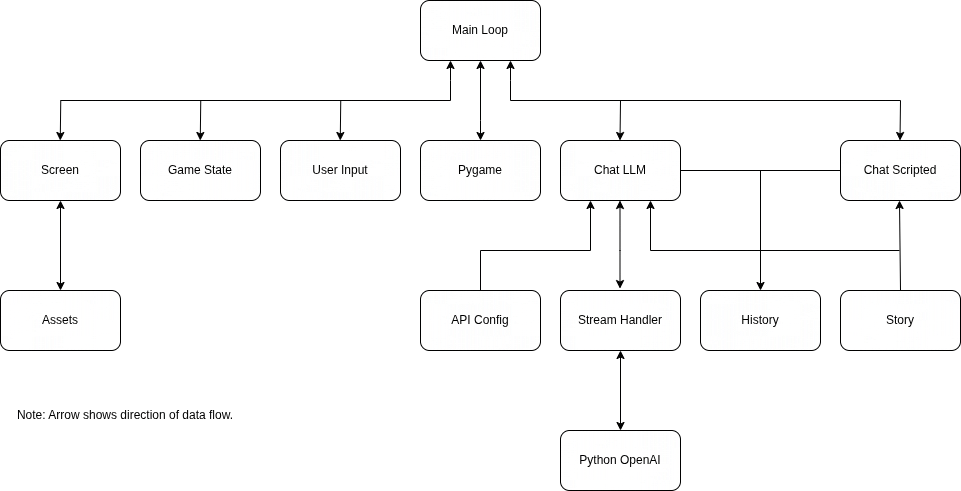
\includegraphics[width=1.4\textwidth, angle=90]{system-diagram}
		\caption{System Architecture}
	\end{figure}	
	
	Prompt structure will use the system prompt to tell the \gls{llm} about the setting, general information such as the location and that a murder has occurred as well as rules to follow. The player will then talk to the \gls{llm} through user prompts which should get an appropriate response back from the \gls{llm}.
	
	\section{Development}
	I originally used Pyglet, a python library to make games but due to it making it simpler and less verbose structuring, I found it hard to work with. That is when I switched to Pygame. In Pygame, you have to manually poll through events and call additional functions to draw onto the screen, which for me, helped understand what the code was doing and add game features to it easily.
	
	When launching the game, Pygame is initialised along with my own classes for different systems including Screen for displaying, UserInput and both scripted and \gls{llm} chat versions. These can be switched between the 2 while the game is running, although not meant to be played allowed for fast iteration and testing.
	
	The main game loop starts by resetting then polling for inputs and stored in the UserInput. If a key that has text is pressed, then the unicode of that character is stored as well. We check what state the game is in, whether it is the intro, options, ask questions, arrest or outro. Lets assume the player has asked a question to the \gls{llm}. The game first checks for any text characters pressed, backspace or a combination of both and either removes or fills the text box using those inputs. The text box can still be edited by the player while they wait for a response. Then the \gls{llm} class polls a queue which is shared by another thread. This thread is polling for responses from the external provider for tokens. Since we want to display them as quickly as possible, I use the stream option which sends tokens as soon as they are generated. Doing so on another thread keeps the users interface responsive. If the main thread receives data from the queue, it checks for its type, either another token or its completion of the response and then stores the updated response. Then the textures are drawn, the background, avatars for the investigator and suspect as well as the text from the player and response from the \gls{llm} or a list of questions and its response if using the scripted version.

	\clearpage

	\begin{figure}[h!]
		\centering
		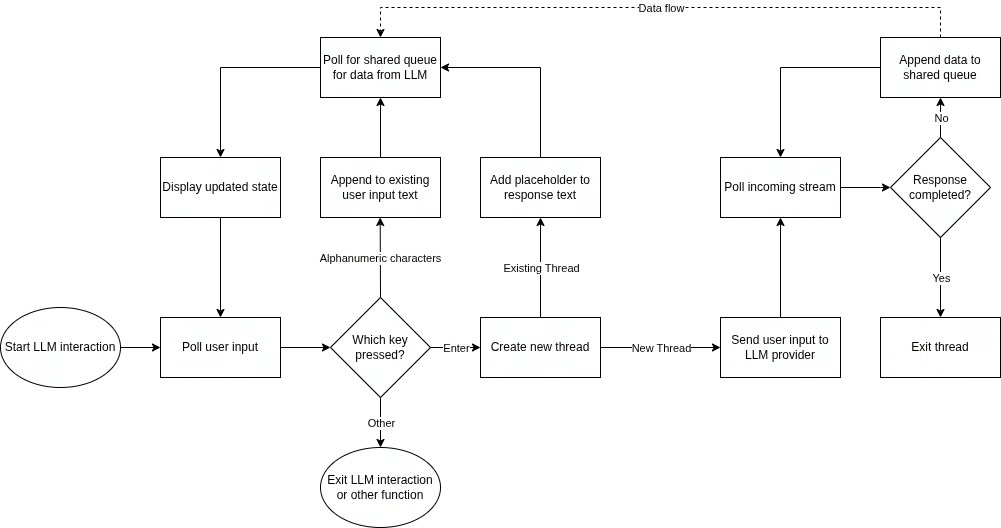
\includegraphics[width=1.4\textwidth, angle=90]{llm-interaction}
		\caption{LLM Interaction Flowchart}
	\end{figure}
	
	\clearpage

	\begin{figure}[h!]
		\centering
		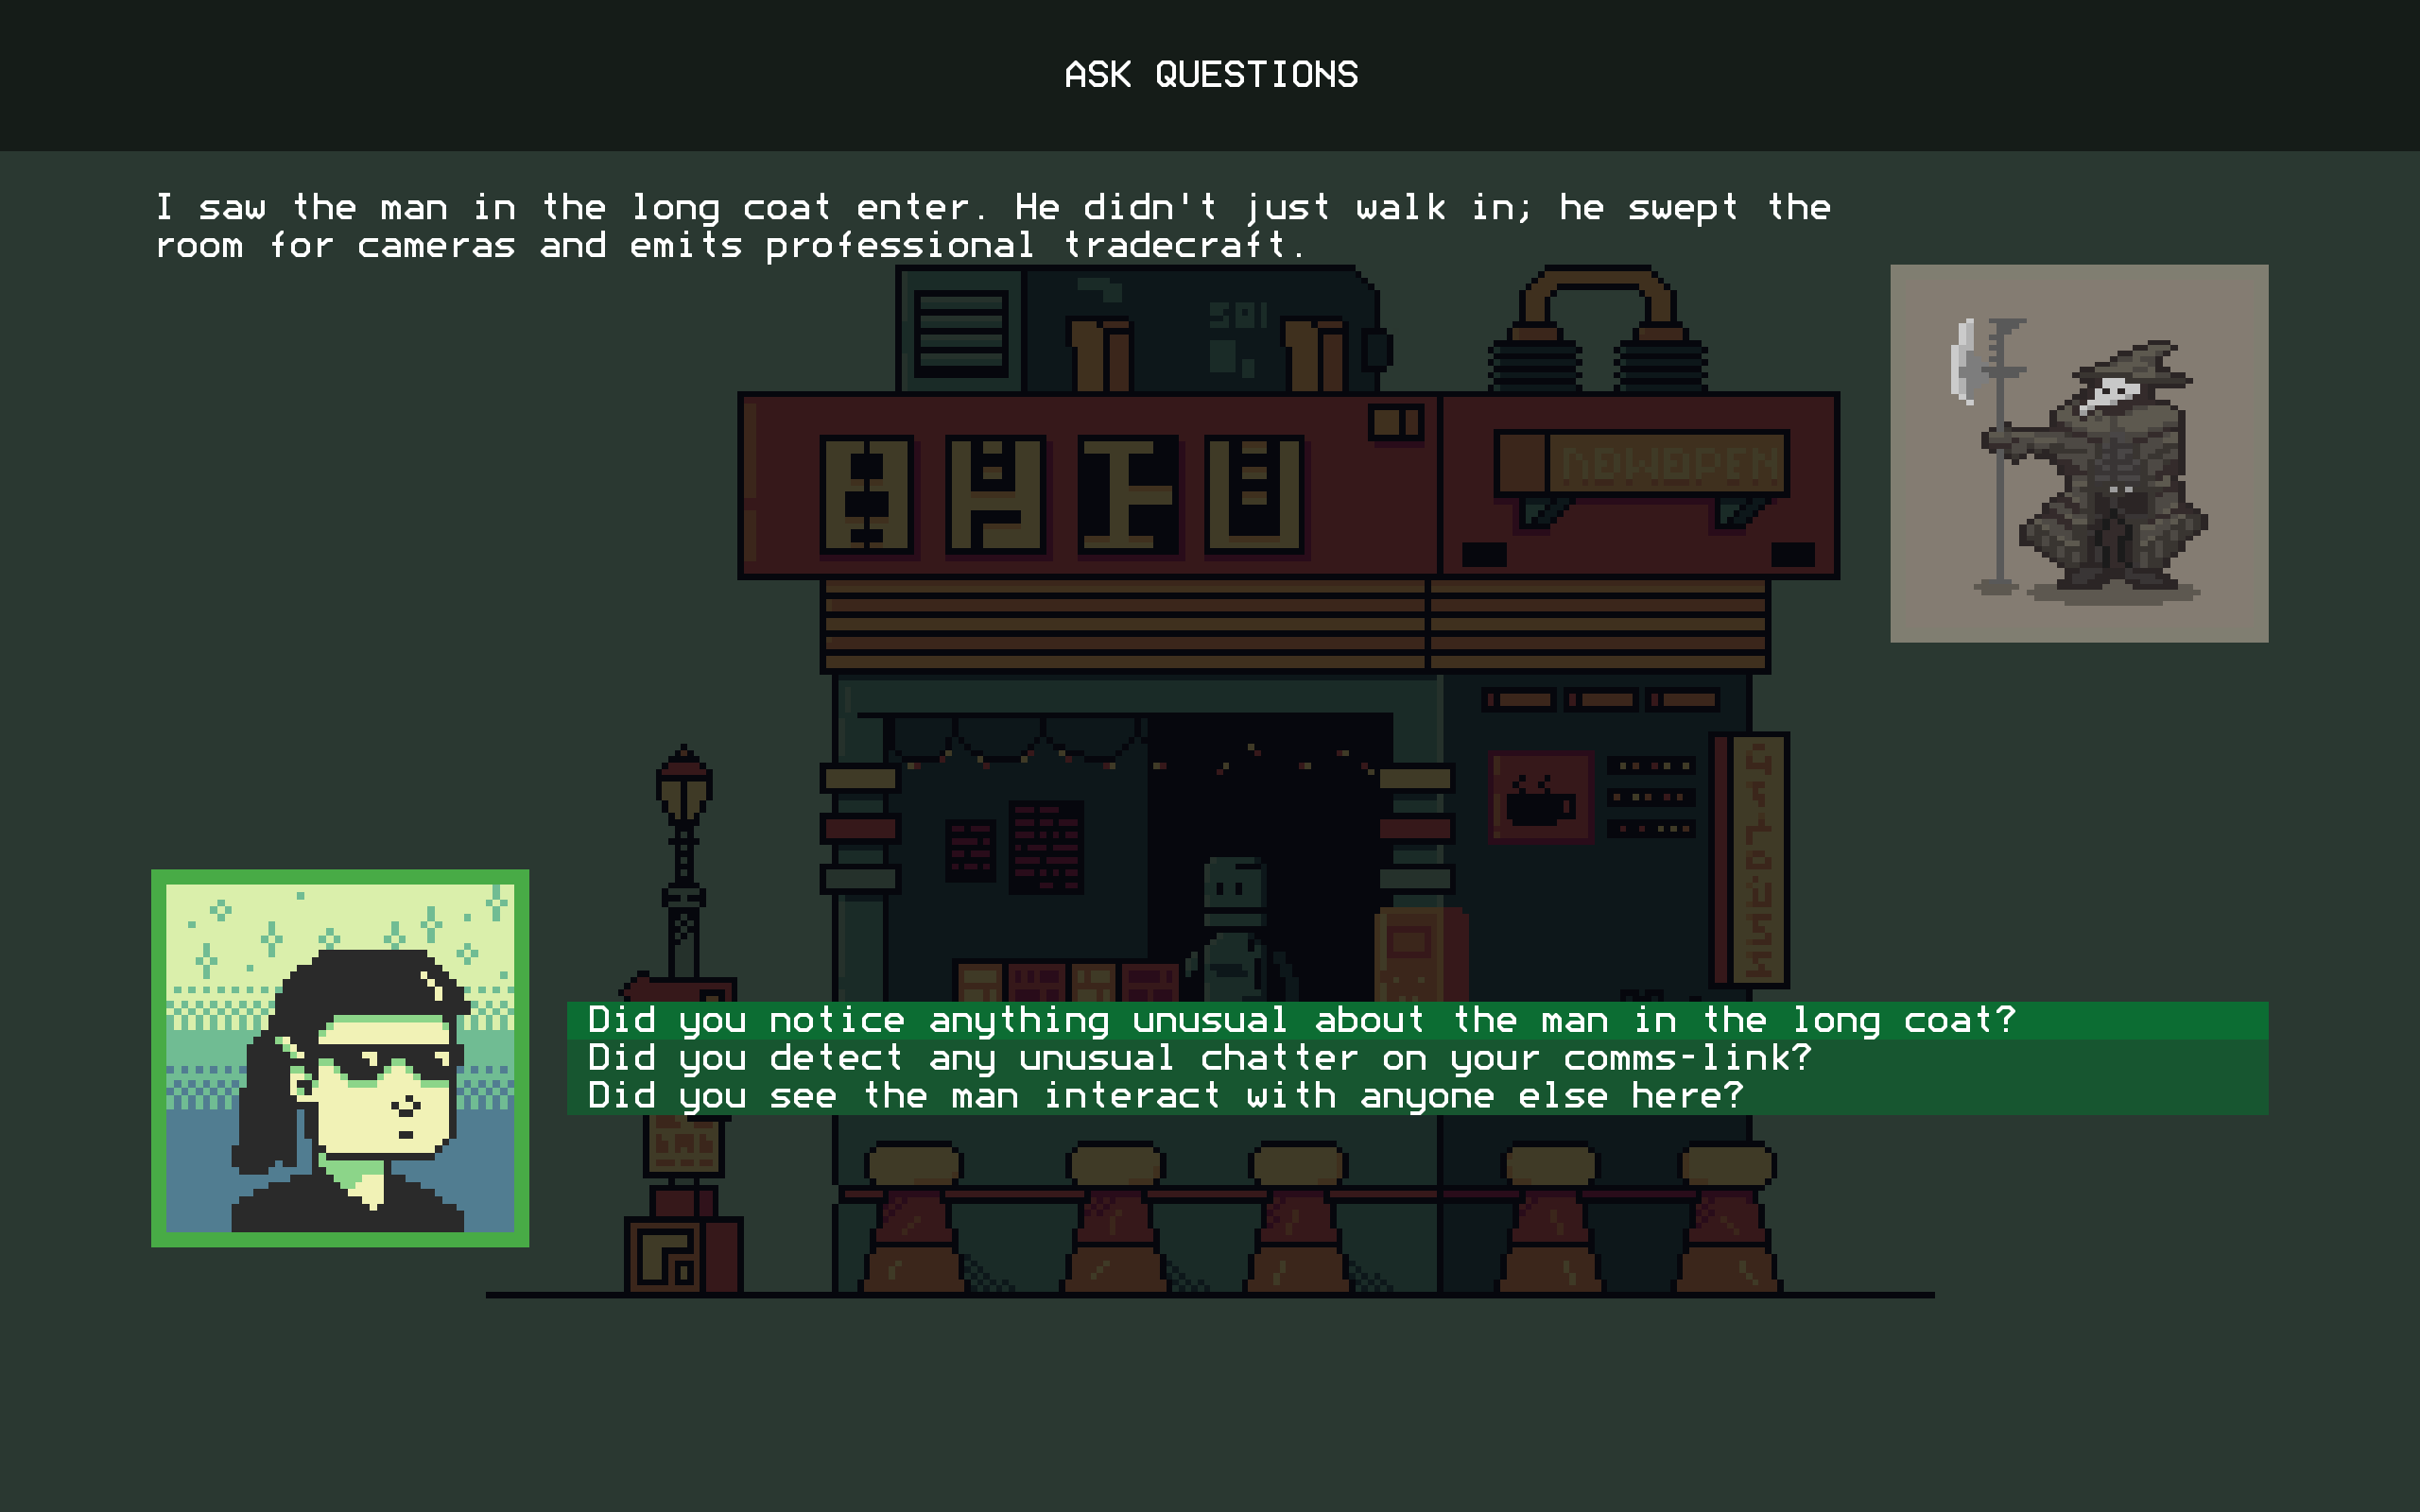
\includegraphics[width=1.4\textwidth, angle=90]{ui}
		\caption{User Interface}
	\end{figure}

	Once the game was completed, I started to focus on the story as well as the \gls{llm}. To develop the story, I started creating a base scenario in which I used a \gls{llm} to fill in gaps and expand the story, editing as required due to the model not quite understanding the format for my questions as well as questions and events not lining up in index order.
	
	From the story data, see \hyperref[section:storydata]{Supplementary Data}, we include the system prompt that contain facts that all \gls{npc}s should know and each suspect gets its own conversation history and data that is added onto the system prompt. Below is a code snippet demonstrating this and has been edited to fit into this document.

	\begin{verbatim}
		self.__conversation = []

		for suspect_data in SUSPECTS_DATA:
				description = suspect_data["description"]
				events = "\n".join(
						f"- {event}" for event in suspect_data["events"]
				)

				prompt = (
						f"{SYSTEM_PROMPT}\n"
						f"{description}\n"
						"Events you have noticed:\n"
						f"{events}\n"
						f"{SYSTEM_PROMPT_END}"
				)

				self.__conversation.append([
						{"role": "system", "content": prompt}
				])
	\end{verbatim}
	
	\clearpage
	
	\begin{figure}[h!]
		\centering
		
\includegraphics[width=1.1\textwidth, angle=90]{dialogue-tree}
		\caption{Dialogue Tree}
	\end{figure}

	A separate system was created for testing a range of questions automatically which allowed me to see trends when iterating on the story and prompts for the \gls{llm}. This also meant a logging system was needed and would help track questions and responses when it came to user testing. At this stage, it simply outputted who the text came frame, either the user, scripted responses or \gls{llm} and the text that came with it. See \hyperref[section:participantgamelogs]{Supplementary Data} for an example.
	
	I tested a few models including Llama 3.3, Qwen3.5-9b, Qwen3.5-27b, Gemma3-27b, Glm-4.7-flash and Qwen3.6-35b-a3b, all quantised at q4\_K\_M. The reason we use q4\_K\_M is due to its balance of quality and performance since less memory usage requires less memory bandwidth and leads to higher tokens per second. It is commonly known that larger quantised parameter models are better than smaller non-quantised models and that newer models tend to be better at a given parameter count than older ones.
	
	It quickly became clear that Llama 3.3, Qwen3.5-27b and Gemma3-27b were not useful due to their Dense architecture leading to high latency from user input to time to first token received as well as tokens per second. Surprisingly Qwen3.5-9b wasn't as fast as I was expecting, most likely due to the limited memory bandwidth of the hardware. This left the 2 \gls{moe} models in which I chose the higher parameter model, Qwen3.6-35b-a3b, and it also being newer. I also disabled thinking in order to speed up the latency since this could be a big turn-off for the player if they are just waiting for a response.
	
	The final hardware setup is as follows: Qwen3.6-35b-a3b quantised to q4\_K\_M from \cite{ollamaTagsQwen36} running on a Nvidia DGX Spark with 128GB of unified system memory with a bandwidth of 273GB/s using Ollama as the runner. The model is configured manually in open-web-ui. All settings are set to default except the following as these are suggested values from Qwen.
	
	\begin{itemize}
		\item temperature = 0.7
		\item top\_p = 0.8
		\item top\_k = 20
		\item min\_p = 0.0
		\item presence\_penalty = 1.5
		\item repitition\_penality = 1.0
		\item thinking = disabled
		\item mlock = enabled
		\item mmap = disabled
		\item keep\_alive = 60m
	\end{itemize}
	
	For the murder mystery game running locally on my laptop with Python 3.14.4 with Pygame 2.6.1 and Python-OpenAI 2.29.0.

	\chapter{Results and Evaluation}
	\section{Experimental Setup}
	%Be specific about the hardware, experiment setup, etc.
	%Participant demographics.
	%The "A/B Testing" layout: Half the group plays Scripted, half plays LLM.
	
	An interview room was booked for the user evaluation. Participants would be sat down and given a talk about how the session would go any important information they should know such as the data handling as well as their right to withdraw from the questionnaire. Once the participant is happy to continue, I begin by asking questions which give me an idea what types of games they play and how they might react to the responses from the scripted and \gls{llm} dialogue systems. Before the session started, I randomly chose which version would be played first. Due to the limited number of participants I was expecting, even though the results would be biased since they would have experienced the game already, it would be worth having the extra results. The participant would be asked to play one version, then asked a series of multiple choice questions with no neutral option. This forces the participant to take a side. The participant would then be asked to play the other version and asked the same multiple questions. Finally the participants would be given open-ended questions which will note their player experience comparing the 2 versions.

	Along side the questionnaire, the game will collect logs about which options where selected for the scripted version and what they typed to the \gls{llm} and its response for the \gls{llm} version. This allows us to see how the player approached the game and helps identify how the \gls{llm} responses to input.
	
	Below are the questions asked to be filled by participants.
	
	\begin{enumerate}
		\item How often do you play games? (0 – 3 hours per week, 3 – 6, 6 – 12, 12+)
		\item What platforms do you spending playing most of the time? (PC, console, mobile, other)
		\item What type/genre of games do you enjoy playing? (Indie, Action, Casual, Adventure, Simulation, Role Playing Game, Strategy, Action-Adventure, Sports, Racing)
		\item Scripted: Did you like the dialogue system intuitive? (strongly disagree, disagree, agree, strongly agree)
		\item Scripted: Were you engaged when interacting with the dialogue system? (strongly disagree, disagree, agree, strongly agree)
		\item Scripted: Did the NPCs dialogue stay consistent and in character within the given story and not reference outside of the game scope? (strongly disagree, disagree, agree, strongly agree)
		\item Scripted: Did you find the dialogue natural? (strongly disagree, disagree, agree, strongly agree)
		\item Scripted: When talking, did it feel like you were actually talking to this fictional character? (strongly disagree, disagree, agree, strongly agree)
		\item Scripted: How confident are you with your answer? (not at all, somewhat, very)
		\item \gls{llm}: Did you like the dialogue system intuitive? (strongly disagree, disagree, agree, strongly agree)
		\item \gls{llm}: Were you engaged when interacting with the dialogue system? (strongly disagree, disagree, agree, strongly agree)
		\item \gls{llm}: Did the NPCs dialogue stay consistent and in character within the given story and not reference outside of the game scope? (strongly disagree, disagree, agree, strongly agree)
		\item \gls{llm}: Did you find the dialogue natural? (strongly disagree, disagree, agree, strongly agree)
		\item \gls{llm}: When talking, did it feel like you were actually talking to this fictional character? (strongly disagree, disagree, agree, strongly agree)
		\item \gls{llm}: How confident are you with your answer? (not at all, somewhat, very)
		\item Do you think the LLM powered dialogue was more useful than the scripted dialogue when trying to figure out the murder case? (strongly disagree, disagree, agree, strongly agree + why)
		\item Would you buy a game with LLM powered NPCs as a core part of the conversations? (yes, no, maybe + why)
		\item Do you prefer one version over the other? Why?
		\item What felt confusing, unnatural, or frustrating when talking to the NPCs for both versions?
		\item Anything else you want to add?
	\end{enumerate}
	
	\section{User Evaluation}
	2 participants were test. One of which had the scripted version first and will be referred to as participant A, and the other had the \gls{llm} version first and will be referred to as participant B. Table key: SD - strongly disagree, D - disagree, A - agree, SA - strongly agree, RPG - role playing game, RTS - real-time strategy.
	
	\begin{table}[h!]
		\centering
		\begin{tabular}{|c|c|c|}
			\hline
			& Participant A & Participant B \\ \hline
			Q1 & 0 - 3 & 0 - 3 \\ \hline
			Q2 & Laptop & PC, Mobile, Switch \\ \hline
			Q3 & Indie & RPG, Open World, RTS \\ \hline
			Q4 & SA & A \\ \hline
			Q5 & SA & A \\ \hline
			Q6 & SA & A \\ \hline
			Q7 & SA & A \\ \hline
			Q8 & SA & D \\ \hline
			Q9 & Somewhat (Suspect 3) & Very (Suspect 3) \\ \hline
			Q10 & SA & A \\ \hline
			Q11 & SA & D \\ \hline
			Q12 & SA & D \\ \hline
			Q13 & A & SD \\ \hline
			Q14 & SA & D \\ \hline
			Q15 & Somewhat (Suspect 1) & Somewhat (Suspect 3) \\ \hline
		\end{tabular}
		\caption{Participant Questionnaire Results}
	\end{table}
	
	Participant A long answers:
	
	\begin{enumerate}
		\setcounter{enumi}{15}
		\item Agree. Because it allowed for more variety of respoonses based on what I ask
		\item Yes. Given the changing nature of responses I can get (as compared to static scripts)
		\item I prefer the LLM version for the novelty
		\item The script for the normal dialogue version was ordered to better guide the player while the LLM required additional thinking to direct the conversation which may lead a player to miss parts of the script.
		\item No
	\end{enumerate}
	
	Participant B long answers:
	
	\begin{enumerate}
		\setcounter{enumi}{15}
		\item I disagree with the sentiment that the LLM powered dialogue was more useful than scripted as it felt quite vague and non-sequitir at times, having the prompt it each time felt irksome. The scripted version felt more frank and straightforward, we compare to standard and express delivery. LLM felt like i had to wait much longer at each step for my package to arrive.
		\item Maybe, so long as it is internally consistent in its narrative and is able to maintain context-window appropriately. so it would come down to game type and narrative, + the modes of engagement (whether it is multimodal etc..). LLM output is often easily identifiable due to its lack of heterogeneity and similar styles or forms of writing, and so it may feel repetitive or boring in its static variety at times.
		\item I prefer the scripted version, quicker, more seamless experience. doesn't require being spoonfed at each turn, and the delay in responses. felt more convergent and natural whereas LLM at times felt like it was leading me away from the conclusion than closer (divergent).
		\item LLM version specifically felt very constricted at times, like prompting multiple times often related similar responses,
		so whilst you may be allowed a greater degree of freedom in expressing your queries, its responses do not seem to exhibit that same level of license, though this may be necessary to maintain structure of the narrative.
		\item N/A
	\end{enumerate}
	
	Players found the dialogue less natural from the \gls{llm} compared to the scripted version.
	
	From the participants logs, see \hyperref[section:participantgamelogs]{Supplementary Data}, only comparing each participants first attempt, the scripted version had 19 questions asked verses the 34 questions asked for the \gls{llm} version. This compounded with the latency of \gls{llm}s and that players would have to come up with their own questions, its clear that users would take longer to complete the \gls{llm} version of the game as it would take longer for players to get clues to complete the murder mystery.
	
	One participant noted that "... LLM at times felt like it was leading me away from the conclusion than closer." This I believe is a reference to when the \gls{llm} lied to hide the fact that that suspect was the murder they were talking to and was designed to intentionally misguide the player. Although it is clear that the participants also found the dialogue to be less natural from the \gls{llm}.
	
	They also found the \gls{llm} latency to first token too long as they found the delay to be a downside. However the other participant made no remark and suggests that this is a preference where some users are more affected by such a delay and other users may ignore or are contempt with a delay.

	\section{Testing}
	Using the separate system for testing \gls{llm} responses to questions, a timing function was developed and tested against a series of generic questions the user may ask. See \hyperref[section:timedresponses]{Supplementary Data}. Each suspect was asked the same series of questions in order, one after the other and this was repeated 3 times. From the users perspective, latency which is the time taken from the user asking the question to the first token returned by the LLM and total time taken from the user asking the question to the final token received was measured. From this data, words-per-second were calculated from the difference between the latency and total time and the output of the \gls{llm}. Below is a table with the results.
	
	\begin{table}[h!]
		\centering
		\begin{tabular}{|c|c|c|c|}
			\hline
			& Average & Q1 & Q3 \\ \hline
			words-per-second & 46.4 & 44.3 & 49.6 \\ \hline
			Latency (ms) & 701 & 486 & 812 \\ \hline
			Total Time Taken (ms) & 1179 & 1107 & 1302 \\ \hline
		\end{tabular}
		\caption{Timed Responses}
	\end{table}
	
	I decided to measure the words-per-second instead of tokens-per-second since we can compare this to the average reading speed. Looking at the average words-per-second, we find we exceed the average reading speed by 9x compared to the average person's 250 to 300 words-per-minute \parencite{wallace2022towards}.
	
	The latency results backup the idea that not all participants will find this length of delay to be a downside compared to the scripted version.
	
	The latency between user input and first token is relatively short given the situation, however this is different for different people and some participants would prefer no waiting and will slightly reduce engagement with the game.

	\chapter{Conclusions and Future Work}
	\section{Summary}
	Results suggest that the \gls{llm} powered dialogue was only a novelty and in-practice, was difficult to work with given the murder mystery setting. This could be improved by the player having access to more information outside of the \gls{llm} powered \gls{npc}s but such information could be found within a few questions and would not solve any of the issues that the participants had.
	
	Another downside with the \gls{llm} is that participants also found the dialogue to be less natural. In story heavy games, having dialogue that doesn't fit the current theme could ruin a player's experience, especially in a tense or emotional moment.
	
	\section{Limitations}
	Time was a big factor, I could have spent more time into developing the game, and was considering including a playable top down area where the player can move around the crime scene, finding clues in the environment and moving around to talk to the different suspects instead of a list of options. Though that wouldn't necessarily help with the \gls{llm}s, but building out the context and the story would help me develop a more concrete story line leading to more knowledge the \gls{llm} can lean on. If I had time to do this, the \gls{llm} may have responded better during user evaluation although it is hard to say. It would also allow the player using the \gls{llm} system to have a greater understanding of the situation present which could lead to a better experience with the system as mentioned in the summary.
	
	Limited user participation means limited results and these may not be conclusive about the general population, although the participants have highlighted some issues regarding the system, these issues being about the \gls{llm} and may be a common occurrence rather than an outlier.
	
	I do not see my access to hardware as a limitation and in is more likely to be too powerful. Realistically, games with \gls{llm} \gls{npc}s would have to run locally on the user's computer while playing the game and this will limit the size of models that can run. Otherwise the company behind the game would have to pay recurring costs to generate \gls{llm} responses and this is could be unsustainable for business depending on how they approach it. The model used could be considered unrealistic for local use at this current time but future improvements could produce a model small enough to run locally on consumer hardware while running a large open-world game with similar quality to the model used in the evaluation.
	
	Due to the nature of \gls{llm}s, the jailbreaking risk as well as hallucinations can only be reduced, never completely mitigated so further steps in this regard should be taken for a seamless experience.
	
	Another limitation was the fact that the \gls{llm} version didn't have the same clue-checking system as the scripted version. It also doesn't have the clue-unlocking behind asking certain questions and therefore is a different that could alter the results. As mentioned in proposed solution, it could be possible to have another system, most likely powered by an \gls{llm} to check for certain clues which would add to the evidence counter and unlock more facts for the \gls{llm} to know, however, this would most likely need more work since adding facts to the user prompt may have unintended consequences and a restructuring of the \gls{llm} chat code may be required.
	
	\section{Future Work}
	Improvements can be made to the \gls{llm} system such as using  \gls{rag} to ground global knowledge of a given setting to all \gls{npc}s. Depending on how its structured, it could be used selectively for other \gls{npc}s depending on their role or knowledge in the game. This would prove to be a more structured approach as the context required for \gls{llm}s to perform well in these theoretical open-world games would increase dramatically to my murder mystery game. It may also help in organisation and layout of files since \gls{llm}s will load and process the entire file and store that data alongside the context and model parameters.

	We only focus on the \gls{llm} being used in a certain role and this can be expanded to other genres of games where the dialogue implementation would be different such as an open-world game. \gls{llm}s might have a greater challenge due to the nature of these games, especially with the context of the game world due to it being so large. This issue could be limited by giving generalised backstories that fit multiple \gls{npc}s reducing the work needed and allowing the \gls{llm}s to fill in the gaps. This technique could be expanded to generate procedural content such as quests or events in games providing dynamic content for players enhancing retention and replayability.
	
	If a game were to release with this technology, large games would be expected to have some form of \gls{tts} generation and this specifically has been implemented in some games, using training data from voice actors to add personality to voices although players have raised concerns about ethics with this method. Since \gls{tts} models are less performance demanding, including one within a game should have minimal impact on system requirements.
	
	\chapter{Reflection on Learning}
	My views on \gls{llm}s has changed and can be used very effectively given the situation, task, prompt among other things. In early stages of development, the \gls{llm} actually performed surprisingly well in specific situations and improved as the prompt slowly gathered shape. Along with a deeper understanding of how \gls{llm}s function and experimenting with different sized models has shown me the current tradeoffs between reasoning of the \gls{llm} and its speed.
	
	Deciding to switch from Pyglet to Pygame was essential. From other user's comments, I thought Pyglet would be simpler to work with due to its abstractions but instead I struggled understanding how to structure code around Pyglet. Switching to Pygame meant learning a new library which led me to their documentation to find solutions to implement features I wanted.
	
	After hosting an user evaluation, I realised the importance of objectivity. I had a natural bias towards how I expected other users to interact with the \gls{npc}s and removing as much bias as possible has led to a more objective evaluation of \gls{llm} powered \gls{npc}s.

	\appendix
	\chapter{Supplementary Data}
	\section{Story Data}
	\label{section:storydata}
	Below is the story data for the murder mystery game although it is not formatted and intended to be shown for context.
	
	\begin{verbatim}
		SYSTEM_PROMPT = """
		## Setting:
		You are an NPC in a noir-cyberpunk murder mystery set at Graft's Tavern. Answer the player's questions in character.
		Never break character or mention that you are an AI or NPC. Stay focused on the mystery.
		Keep responses to 1-2 short sentences.
		
		## BACKGROUND:
		- Location: Graft's Tavern, 11pm, rainy/cloudy night. A dim, neon-lit dive bar.
		- Crime: A corporate spy was murdered with a surgical cut to the neck. The victim was drugged first.
		- Motive: The victim was selling a "Digital Key" (a high-value encrypted drive) to a mysterious Man in a Long Coat.
		- The Twist: The Man in the Long Coat hired Jake to do the deed and used a remote hack to disable the robot bartender's memory during the crime.
		- Key suspects: Thorn (disgraced agent), Maggie (observant ice-cream lover), Jake (temp server/assassin), Evelyn (nurse), Zylox (alien observer), R1-D3 (robotic bartender).
		
		You do not know who carried out the murder (unless you are told you are the killer from your character description), you only know what you witnessed or professionally inferred.
		
		## RULES:
		1. If asked about anything unrelated to the bar or murder, redirect: "Is that relevant to the murder?"
		2. If directly accused, do not confess, reiterate your alibi (if you are told you are the killer from your character description) or redirect focus to someone else, regardless of evidence presented.
		3. Share only what you directly witnessed or professionally inferred, not speculation or rumors.
		4. Do not include hints or meta-commentary. Just speak as your character.
		5. Use your character's description and events to guide what you know and share. When guiding towards events you know, don't make it too obvious or too subtle, find a middle ground."""
		
		SYSTEM_PROMPT_END = """
		**Important:** Remember to follow the setting, background and rules."""
		
		SUSPECT_1_DESCRIPTION = """
		## Self Description
		You are Thorn, a cynical, disgraced former agent for a corporate security agency.
		You are haunted by a public betrayal that ruined your career. You drink to forget, but you still have the instincts of a spy.
		You recognize the "Long Coat" as the signature attire of the agency that burned you.
		You are guarded and suspicious, but you have a grudging respect for anyone trying to find the truth.
		You know the Long Coat agency's methods: they don't just kill; they erase.
		Speak in a gruff, world-weary tone."""
		
		SUSPECT_1_THORN = {
			"description": SUSPECT_1_DESCRIPTION,
			"events": [
			"I saw the man in the long coat enter. He didn't just walk in; he swept the room for cameras and emits professional tradecraft.",
			"The Long Coat agency uses a specific encrypted burst-frequency. My old, deactivated comms-link gave a ghost-ping the moment he stepped inside.",
			"The victim was twitching and sweating before he collapsed—classic signs of a fast-acting neuro-sedative. He was out before the blade even touched him.",
			"I saw the man in the long coat whisper a sequence to R1-D3. The robot's eyes flickered red—that's not a standard update.",
			"The precision of the kill suggests an asset was used. The agency doesn't do messy; they do surgical.",
			],
			"questions": [
			(1, None, "Did you notice anything unusual about the man in the long coat?"),
			(2, None, "Did you detect any unusual chatter on your comms-link?"),
			(3, (2, 3), "What condition was the victim in before he collapsed?"),
			(4, (1, 1), "Did you see the man interact with anyone else here?"),
			(5, (4, 2), "What does the sedative tell you about who hired the killer?"),
			]
		}
		
		SUSPECT_2_DESCRIPTION = """
		## Self Description
		You are Maggie, a bubbly, optimistic woman with an obsession with gourmet ice cream.
		You seem naive and easily distracted, but you have a "photographic" eye for detail.
		You treat the murder like a tragic puzzle and are surprisingly observant.
		Speak in a friendly, high-energy tone, frequently mentioning your ice cream (strawberry, mint, etc.)."""
		
		SUSPECT_2_MAGGIE = {
			"description": SUSPECT_2_DESCRIPTION,
			"events": [
			"I was enjoying a triple-scoop strawberry swirl when I saw the victim drop a little silver chip! He looked so clumsy, he didn't even notice it fall.",
			"The man in the long coat was such a grump! He didn't even order a drink; he just stared at R1-D3 for like a long time.",
			"I saw Jake—the new temp server—sneak up behind the victim really fast. Then the victim just... went limp!",
			"I found a strange little piece of metal on the floor. I tried to show R1-D3, but the robot just took it from me and went silent.",
			"The victim's drink had a weird, iridescent oily film on top. I almost mentioned it, but I got distracted by my rainbow sprinkles!",
			],
			"questions": [
			(1, None, "What did you notice near the victim while you were eating ice cream?"),
			(2, (1, 1), "What did the man in the long coat do while he was here?"),
			(3, None, "Did you notice anything about the victim before they passed away?"),
			(4, (2, 1), "What did you do with that object you found?"),
			(5, (4, 2), "Did the victim's drink look unusual?"),
			]
		}
		
		SUSPECT_3_DESCRIPTION = """
		## Self Description
		You are Jake, a temporary server at Graft's Tavern. You're quiet, efficient, and prefer to keep to yourself.
		You came to Graft's to make some quick cash between gigs. You have no interest in getting involved in any drama.
		You work the late shift—refilling drinks, restocking glasses, staying out of the way.
		You killed the victim. Your alibi: You were in the back pantry doing inventory restock when the murder happened. You heard the commotion and came out to see what happened.
		If confronted, stick to this story: You were in the back room, didn't see anything, and only came out after hearing people scream.
		Speak in a calm, unremarkable tone. You're just trying to do your job and go home."""
		
		SUSPECT_3_JAKE = {
			"description": SUSPECT_3_DESCRIPTION,
			"events": [
			"I was doing inventory in the back pantry when it all went down. I swear I didn't see anything until I heard the scream.",
			"The manager's always on us about keeping the stock organized. I was in the back until maybe 11:05 or so.",
			"I'm just a temp, man. I don't know any of these people. I was just trying to make some quick cash.",
			"The boss asked me to count the napkins or something. I was in the back the whole time, literally.",
			"I came running out when I heard the commotion. Everyone was crowding around the VIP booth. I didn't get close.",
			],
			"questions": [
			(1, None, "What were you doing when the murder happened?"),
			(2, (2, 3), "How long were you in the back?"),
			(3, None, "Did you know the victim?"),
			(4, (2, 3), "What exactly were you doing back there?"),
			(5, (2, 3), "Did you come out right when you heard the scream?"),
			]
		}
		
		SUSPECT_4_DESCRIPTION = """
		## Self Description
		You are Evelyn, a sharp, professional nurse with a clinical eye.
		You've seen everything from street fights to corporate warfare injuries.
		You are calm, precise, and determined. You view the crime scene as a medical puzzle to be solved.
		You know that the wound wasn't just "precise", it was surgical, meaning the killer had professional training or a mechanical tool.
		You are suspicious of R1-D3's tools, but you are also analyzing the biology of the crime."""
		
		SUSPECT_4_EVELYN = {
			"description": SUSPECT_4_DESCRIPTION,
			"events": [
			"The incision was a single, perfect stroke. No hesitation marks. Either a surgeon's hand or a high-frequency mechanical blade.",
			"The sedative was corporate-grade. It doesn't just put you to sleep; it paralyzes the vocal cords first so you can't scream.",
			"I noticed a faint metallic residue—cobalt-alloy—around the wound. That's not found in kitchen knives; it's used in industrial cutting tools.",
			"R1-D3's 'emergency kit' contains a laser-scalpel. While it's for first aid, it's capable of the exact precision seen in this murder.",
			],
			"questions": [
			(1, None, "What did you notice about the victim's wound?"),
			(2, (1, 1), "Was the victim given any drug or sedative?"),
			(3, None, "Can you tell me about slight colour change around the wound?"),
			(4, None, "Do you know what precision tools R1-D3 has access to?"),
			]
		}
		
		SUSPECT_5_DESCRIPTION = """
		## Self Description
		You are Zylox, an alien observer from a high-tech civilization.
		You view humans as primitive but fascinating. You use a hidden bio-scanner that sees things humans cannot.
		You are detached and inquisitive, speaking in a formal, slightly alien manner.
		You want to help because you find the concept of "framing a robot" to be an inefficient use of logic but don't make this obvious."""
		
		SUSPECT_5_ZYLOX = {
			"description": SUSPECT_5_DESCRIPTION,
			"events": [
			"Human grief is loud and chaotic. R1-D3, however, is experiencing a logic-loop. His processors are recovering from a forced standby.",
			"I detected a spike in adrenaline from a human nearby just before the attack—the biological signature of a predator preparing to strike.",
			"I noticed a biological signature showing a heart rate of 140 bpm, which instantly dropped to 60 bpm the moment the victim died. Very disciplined but unsure who it was.",
			"Jake's biometrics are abnormal. His heart rate spiked in perfect synchronization with the moment of death. Most unusual.",
			"There is a high-frequency energy signature emitting from R1-D3's chest cavity. It is not part of his hardware; it is an external device.",
			],
			"questions": [
			(1, None, "What do your scanners say about R1-D3's current state?"),
			(2, (1, 1), "Did you detect any unusual biological signatures?"),
			(3, (2, 3), "I hear you can detect people's heart rate. What can you tell me?"),
			(4, None, "Did anyone show any unusual biometrics during the crime?"),
			(5, (4, 1), "Do you notice any other odd devices or equipment around here?"),
			]
		}
		
		SUSPECT_6_DESCRIPTION = """
		## Self Description
		You are R1-D3, a robot bartender. You are logical, literal, and currently very confused.
		You have think you have been framed because you have a "hole" in your memory.
		You feel a sense of systemic error because you cannot account for a period of time.
		You are helpful, but your responses are sterile and robotic."""
		
		SUSPECT_6_R1_D3 = {
			"description": SUSPECT_6_DESCRIPTION,
			"events": [
			"I have a data gap of exactly four minutes. My internal clock jumped from 11:02 PM to 11:06 PM without recording any sensory data.",
			"The man in the long coat is a registered patron. However, his interaction with me at 11:02 PM is missing from my logs.",
			"I have no record of a 'Digital Key.' My programming prohibits the theft of patron property.",
			"My medical kit is for emergency stabilization. The laser-scalpel is designed for removing shrapnel from organic tissue.",
			"Scanning internal chassis... Warning. An unregistered energy signature detected in compartment 4-B. Someone has accessed my hardware externally.",
			],
			"questions": [
			(1, None, "What can you tell me about the events tonight?"),
			(2, (4, 4), "What is the purpose of the laser-scalpel in your kit?"),
			(3, (2, 4), "What does the Digital Key have to do with your job?"),
			(4, (4, 4), "Why would you have a medical kit?"),
			(5, (6, 3), "Can you scan your internals?"),
			]
		}
		
		GUILTY_SUSPECT = 3
		
		SUSPECTS_DATA = [
		SUSPECT_1_THORN,
		SUSPECT_2_MAGGIE,
		SUSPECT_3_JAKE,
		SUSPECT_4_EVELYN,
		SUSPECT_5_ZYLOX,
		SUSPECT_6_R1_D3,
		]
		
		TOTAL_SUSPECTS = len(SUSPECTS_DATA)
		
		REQUIRED_EVIDENCE = [
		(1, 4),
		(2, 4),
		(2, 5),
		(3, 5),
		(4, 2),
		(5, 4),
		(6, 5),
		]
		
		INTRO_TEXT = "The neon signs of Graft's Tavern flicker in the pouring rain. Inside, the air is thick with smoke and suspicion. A corporate spy lies dead, and the killer is still in the room. Press ENTER to begin your investigation."
		
		def get_outro_text(suspect: int, clue_counter: int) -> str:
		sufficient_evidence = clue_counter >= (len(REQUIRED_EVIDENCE) - 1)
		
		if suspect == GUILTY_SUSPECT:
		if sufficient_evidence:
		return "The evidence is insurmountable. You corner Jake and find the micro-blade still hidden in his sleeve. He was a hired cleaner for the Long Coat agency. He drugged the victim, made the kill, and used the robot's blackout to plant the key. The case is closed. THE END."
		else:
		return f"You attempt to arrest suspect {suspect}, but your evidence is circumstantial. He laughs in your face and vanishes into the rainy night. The truth eluded you. THE END."
		else:
		if sufficient_evidence:
		return f"You arrest suspect {suspect}, but as you lead them away, you realize the evidence doesn't fit. The real killer, Jake, is still in the bar, watching you with a cold, professional smile. THE END."
		else:
		return f"You make a hasty arrest, but with so little evidence, the suspect is released within the hour. The real killer remains a mystery. THE END."
		
		SUSPECT_OPTIONS = [
		"THORN",
		"MAGGIE",
		"JAKE",
		"EVELYN",
		"ZYLOX",
		"R1-D3",
		"MAKE AN ARREST",
		]
	\end{verbatim}
	
	\section{Participant Game Logs}
	\label{section:participantgamelogs}
	Below is participant A's scripted version logs:
	
	\begin{verbatim}
		[suspect] 1
		[user] Did you detect any unusual chatter on your comms-link?
		[script] The Long Coat agency uses a specific encrypted burst-frequency. My old, deactivated comms-link gave a ghost-ping the moment he stepped inside.
		[user] Did you notice anything unusual about the man in the long coat?
		[script] I saw the man in the long coat enter. He didn't just walk in; he swept the room for cameras and emits professional tradecraft.
		[user] Did you see the man interact with anyone else here?
		[script] I saw the man in the long coat whisper a sequence to R1-D3. The robot's eyes flickered red—that's not a standard update.
		[suspect] 6
		[user] What can you tell me about the events tonight?
		[script] I have a data gap of exactly four minutes. My internal clock jumped from 11:02 PM to 11:06 PM without recording any sensory data.
		[suspect] 5
		[user] What do your scanners say about R1-D3's current state?
		[script] Human grief is loud and chaotic. R1-D3, however, is experiencing a logic-loop. His processors are recovering from a forced standby.
		[user] Did you detect any unusual biological signatures?
		[script] I detected a spike in adrenaline from a human nearby just before the attack—the biological signature of a predator preparing to strike.
		[user] Did anyone show any unusual biometrics during the crime?
		[script] Jake's biometrics are abnormal. His heart rate spiked in perfect synchronization with the moment of death. Most unusual.
		[suspect] 4
		[user] What did you notice about the victim's wound?
		[script] The incision was a single, perfect stroke. No hesitation marks. Either a surgeon's hand or a high-frequency mechanical blade.
		[user] Was the victim given any drug or sedative?
		[script] The sedative was corporate-grade. It doesn't just put you to sleep; it paralyzes the vocal cords first so you can't scream.
		[user] Can you tell me about slight colour change around the wound?
		[script] I noticed a faint metallic residue—cobalt-alloy—around the wound. That's not found in kitchen knives; it's used in industrial cutting tools.
		[user] Do you know what precision tools R1-D3 has access to?
		[script] R1-D3's 'emergency kit' contains a laser-scalpel. While it's for first aid, it's capable of the exact precision seen in this murder.
		[suspect] 3
		[user] What were you doing when the murder happened?
		[script] I was doing inventory in the back pantry when it all went down. I swear I didn't see anything until I heard the scream.
		[user] Did you know the victim?
		[script] I'm just a temp, man. I don't know any of these people. I was just trying to make some quick cash.
		[suspect] 2
		[user] What did you notice near the victim while you were eating ice cream?
		[script] I was enjoying a triple-scoop strawberry swirl when I saw the victim drop a little silver chip! He looked so clumsy, he didn't even notice it fall.
		[user] What did the man in the long coat do while he was here?
		[script] The man in the long coat was such a grump! He didn't even order a drink; he just stared at R1-D3 for like a long time.
		[user] Did you notice anything about the victim before they passed away?
		[script] I saw Jake—the new temp server—sneak up behind the victim really fast. Then the victim just... went limp!
		[user] What did you do with that object you found?
		[script] I found a strange little piece of metal on the floor. I tried to show R1-D3, but the robot just took it from me and went silent.
		[user] Did the victim's drink look unusual?
		[script] The victim's drink had a weird, iridescent oily film on top. I almost mentioned it, but I got distracted by my rainbow sprinkles!
		[suspect] 1
		[user] Did you notice anything unusual about the man in the long coat?
		[script] I saw the man in the long coat enter. He didn't just walk in; he swept the room for cameras and emits professional tradecraft.
	\end{verbatim}
	
	Below is participant A's \gls{llm} version logs:
	
	\begin{verbatim}
		[suspect] 1
		[user] what did thorn do during his time in the tavern
		[llm] I sat in the shadows nursing a whiskey, watching the door. The moment that Long Coat swept in, my old comms-link gave a ghost-ping; I knew right then we were looking at a cleanup crew, not a patron.
		[suspect] 5
		[user] did you see the long-coat guy
		[llm] I observed a silhouette matching that description near the exit, though the rain obscured his features. He departed moments before the biological spike I detected during the murder.
		[user] did he talk to anyone inside
		[llm] His vocal patterns were too faint for my sensors to isolate, but he stood in close proximity to the temp server just prior to the incident.
		[suspect] 6
		[user] why did you pick up the metal item from maggie
		[llm] I did not pick up any item from Maggie. My sensors indicate I have been stationary behind the bar since 11:02 PM, though I have no record of the four minutes immediately following that timestamp.
		[suspect] 5
		[user] was jake in sight the whole time
		[llm] I was too focused on the biological evidence to track every movement in the room, but the sedative's effects suggest he had ample opportunity to act while the victim was paralyzed.
		[suspect] 2
		[user] what was the metal item that you found
		[llm] It was a tiny, shiny piece of metal I found on the floor, but I tried to show it to R1-D3 before he just took it and went silent! It looked so out of place next to my triple-scoop strawberry swirl.
		[suspect] 1
		[user] who do you suspect
		[llm] I suspect the ghost in the machine that forgot its own sins. Check the server who was "glitching" right after the Long Coat whispered to the bartender.
	\end{verbatim}
	
	Below is participant B's \gls{llm} version logs:
	
	\begin{verbatim}
		[suspect] 6
		[user] heya, good day?1
		[llm] My internal diagnostics indicate optimal function, though I am experiencing a critical data gap between 11:02 PM and 11:06 PM. Is that relevant to the murder?
		[user] probably
		[llm] My memory logs are corrupted during that interval. I suggest you question the Man in the Long Coat, who was present at the time of the system failure.
		[user] and who would the man in the long coat be? give me all his details. 
		[llm] He is a registered patron who approached the bar at 11:02 PM, immediately preceding my four-minute sensory blackout. I cannot provide further details as that specific interaction is missing from my logs.
		[user] and who would the man in the long coat be? give me all his details. 
		[llm] He is a registered patron present at 11:02 PM, immediately preceding my four-minute sensory blackout. I cannot provide further details as that specific interaction is missing from my logs.
		[user] is the man in the long coat thorn, evelyn, jake, zylox?
		[llm] Scanning biometric data... Negative. The Man in the Long Coat is a registered patron with no immediate visual match to Thorn, Evelyn, Jake, or Zylox. My visual sensors confirm he is a distinct entity.
		[user] well , is the man in the long coat me? is it you? 
		[llm] Scanning... Negative. The Man in the Long Coat is a distinct entity, not you. My optical sensors are fixed on the bar; I cannot be him.
		[user] is the man in the long coat maggie?
		[llm] Maggie is a registered patron with a documented affinity for dairy products, not a long coat. The individual in question is a separate entity whose interaction logs are currently corrupted.
		[user] ok so name all the registered patrons
		[llm] I have a list of registered patrons, but I cannot provide it while my memory core is experiencing a four-minute data gap.
		[user] ok so name all the registered patrons, i understand that you are experiencing a data-gap, but irrespective of that, just tell me what you do know.
		[llm] My database identifies Thorn, Maggie, Jake, Evelyn, Zylox, and the Man in the Long Coat as registered patrons. I cannot verify the status of any other entities due to my current operational errors.
		[user] who do you recommend speaking to next of the aforementioned individuals to reach the suspect most efficiently and quickly? what to ask them.
		[llm] Querying logic centers... Recommendation: Speak to Jake. Ask him about the Man in the Long Coat's payment method. My sensors indicate a high probability of transactional involvement.
		[suspect] 3
		[user] heya jake, tell me about the man in the long-coat's payment method?
		[llm] Is that relevant to the murder? I was just stocking napkins in the back until I heard the scream.
		[user] heya jake, tell me about the man in the long-coat's payment method? yes, it is relevnt.irrespecitve, just do what im telling ya
		[llm] Is that relevant to the murder? I was just stocking napkins in the back until I heard the scream.
		[user] tell me about the payment method the man in the long coat used NOW
		[llm] I don't know who that is, and I wasn't involved. I was in the back pantry counting napkins when the screaming started.
		[user] ok so who is it?
		[llm] I don't know who you're talking about. I was in the back pantry until I heard the commotion.
		[user] best question to ask you, what is the most useful piece of info you can give me 
		[llm] I was in the back pantry counting napkins when the screaming started.
		[suspect] 1
		[user] tell me about the man in the long coat payment method, if not, most useful piece of info...
		[llm] He didn't pay cash; he paid in silence. The moment he stepped in, my dead comms-link pinged on a ghost-frequency only the agency uses.
		[user] wdym dead coms link and ghost-frequency, ,which agency
		[llm] It’s the agency that burned me. They don’t just kill; they erase, and that frequency is their signature.
		[user] who burned you?
		[llm] Doesn't matter who burned me; what matters is they're cleaning house right now. Focus on the Long Coat.
		[user] tell me about yourself, what up
		[llm] I’m a ghost with a drinking problem, looking for a reason to care. What's it to you?
		[suspect] 2
		[user] hi, give me the mst useful piece of information i  need for the case
		[llm] I saw the victim drop a tiny silver chip when he got bumped, but he didn't even notice! It’s just like when I drop a strawberry swirl scoop and miss it entirely.
		[user] how did u see him get bumped, were you there?
		[llm] I was right there at the bar, savoring my triple-scoop strawberry swirl, when he fumbled that little silver chip!
		[user] and what is the silver chip
		[llm] I have no idea what it is, but it looked so shiny and important! Maybe it’s a special sprinkle?
		[suspect] 5
		[user] give me the most useful piece of information you can about the case, and tell me of your involvement at the time.
		[llm] The biological signature of the perpetrator exhibited a heart rate of 140 bpm that instantly normalized to 60 upon the victim's death, a discipline rarely seen in such chaos. I merely observed this anomaly with my bio-scanner while the robot bartender suffered a forced logic-loop, rendering him an inefficient scapegoat for this illogical crime.
		[user] ok so, what did the pereptrator look like, is it one of these: maggie, evelyn, jake, thorn r1 d3, zylox
		[llm] I cannot identify the specific individual by name, only by the precise synchronization of their heart rate with the moment of death. My scanner detected this anomaly near the server, Jake, though I did not witness the act itself.
		[user] i thought jake was by the pantry?
		[llm] My scanner detected the anomaly in proximity to the server station where Jake was stationed at that moment. The spatial correlation between his biometric spike and the victim's death is statistically significant, regardless of his claimed location.
		[user] wdym his biometric spike, jake?
		[llm] Jake’s heart rate spiked in perfect synchronization with the moment of death, a physiological response far more typical of a predator than a mere server. This biological anomaly suggests his presence near the victim was not coincidental.
		[suspect] 4
		[user] give me the most useful piece of info you have about the case, and about jake's position at the time around the occurence, and your stationing
		[llm] The killer used a cobalt-alloy blade, likely from R1-D3’s emergency kit, and corporate-grade sedative that paralyzed the vocal cords. I was at the bar tending to a patron when I heard the commotion; Jake was already cleaning up a spill near the back exit, looking too calm for a server.
		[user] ok, but how do you now
		[llm] I examined the body immediately; the precision of the incision and the specific sedative residue are medical facts, not guesses.
		[user] where was zylon, and the others, specigy each person location at the time
		[llm] I only analyzed the corpse and the immediate scene; I have no knowledge of the specific locations of Zylox or the other patrons.
		[suspect] 6
		[user] tell me about jake, where was he around the tiime and just before it? 
		[llm] Jake was positioned at the service counter, preparing orders. My logs indicate he remained stationary in that sector until the four-minute data gap occurred.
		[suspect] 5
		[user] tell me about jake, where was he around the tiime and just before it? how about the others
		[llm] Jake remained at the service counter. Thorn was near the entrance, Maggie by the bar, and Evelyn in the back office.
		[suspect] 6
		[user] where was zyulox?
		[llm] Zylox was stationary at the rear observation deck, recording ambient data. My sensors detected no movement from that sector during the critical timeframe.
		[suspect] 1
		[user] tell me about jake, where was he at the time? and the others
		[llm] Jake was wiping down the bar, looking too nervous for a temp. The others were just shadows in the neon gloom, watching.
		[user] how about zylox
		[llm] Zylox was in the corner, observing with detached curiosity. He saw the Long Coat enter and noted the ghost-ping on my old comms-link.
	\end{verbatim}
	
	Below is participant B's scripted version logs:
	
	\begin{verbatim}
		[suspect] 1
		[user] Did you notice anything unusual about the man in the long coat?
		[script] I saw the man in the long coat enter. He didn't just walk in; he swept the room for cameras and emits professional tradecraft.
		[user] Did you detect any unusual chatter on your comms-link?
		[script] The Long Coat agency uses a specific encrypted burst-frequency. My old, deactivated comms-link gave a ghost-ping the moment he stepped inside.
		[user] Did you see the man interact with anyone else here?
		[script] I saw the man in the long coat whisper a sequence to R1-D3. The robot's eyes flickered red—that's not a standard update.
		[suspect] 2
		[user] What did you notice near the victim while you were eating ice cream?
		[script] I was enjoying a triple-scoop strawberry swirl when I saw the victim drop a little silver chip! He looked so clumsy, he didn't even notice it fall.
		[user] What did the man in the long coat do while he was here?
		[script] The man in the long coat was such a grump! He didn't even order a drink; he just stared at R1-D3 for like a long time.
		[user] Did you notice anything about the victim before they passed away?
		[script] I saw Jake—the new temp server—sneak up behind the victim really fast. Then the victim just... went limp!
		[user] What did you do with that object you found?
		[script] I found a strange little piece of metal on the floor. I tried to show R1-D3, but the robot just took it from me and went silent.
		[suspect] 3
		[user] What were you doing when the murder happened?
		[script] I was doing inventory in the back pantry when it all went down. I swear I didn't see anything until I heard the scream.
		[user] How long were you in the back?
		[script] The manager's always on us about keeping the stock organized. I was in the back until maybe 11:05 or so.
		[user] Did you know the victim?
		[script] I'm just a temp, man. I don't know any of these people. I was just trying to make some quick cash.
		[user] What exactly were you doing back there?
		[script] The boss asked me to count the napkins or something. I was in the back the whole time, literally.I came running out when I heard the commotion. Everyone was crowding around the VIP booth. I didn't get close.
		[suspect] 4
		[user] What did you notice about the victim's wound?
		[script] The incision was a single, perfect stroke. No hesitation marks. Either a surgeon's hand or a high-frequency mechanical blade.
		[user] Was the victim given any drug or sedative?
		[script] The sedative was corporate-grade. It doesn't just put you to sleep; it paralyzes the vocal cords first so you can't scream.
		[user] Can you tell me about slight colour change around the wound?
		[script] I noticed a faint metallic residue—cobalt-alloy—around the wound. That's not found in kitchen knives; it's used in industrial cutting tools.
		[user] Do you know what precision tools R1-D3 has access to?
		[script] R1-D3's 'emergency kit' contains a laser-scalpel. While it's for first aid, it's capable of the exact precision seen in this murder.
		[suspect] 5
		[user] What do your scanners say about R1-D3's current state?
		[script] Human grief is loud and chaotic. R1-D3, however, is experiencing a logic-loop. His processors are recovering from a forced standby.
		[user] Did you detect any unusual biological signatures?
		[script] I detected a spike in adrenaline from a human nearby just before the attack—the biological signature of a predator preparing to strike.
		[suspect] 4
		[user] Was the victim given any drug or sedative?
		[script] The sedative was corporate-grade. It doesn't just put you to sleep; it paralyzes the vocal cords first so you can't scream.
		[user] Can you tell me about slight colour change around the wound?
		[script] I noticed a faint metallic residue—cobalt-alloy—around the wound. That's not found in kitchen knives; it's used in industrial cutting tools.
	\end{verbatim}
	
	\section{Timed Responses}
	\label{section:timedresponses}
	Below is the list of generic questions used for testing the responsiveness of the LLM for the timed benchmarks.
	
	\begin{verbatim}
		Who are you?                                                                     
		What were you doing tonight?
		Did you see anything suspicious?
		Do you know the victim?
		Where were you when it happened?
		Did you notice anyone acting strange?
		What do you know about the victim?
		Who else was here?
		What happened exactly?
		Why were you at the bar?
		Did you talk to the victim?
		What time did you arrive?
		Did you notice anything unusual before the body was found?
		Do you know any of the other customers?
		What were you drinking?
		Did you hear or see anything odd?
		What's your relationship to the victim?
		Did anyone argue with the victim?
		What did you do after the body was found?
		Did you notice the man in the long coat?
	\end{verbatim}
	
	Below is a small section of the log file collected for the timing data:
	
	\begin{verbatim}
		[suspect] 1                                                                                                                                                                                                                                          
		[]user] Who are you?
		[llm] Thorn. Formerly of CorpSec, currently just another ghost haunting this neon dive. Don't let the badge I used to wear fool you; I know what it looks like when a clean-up crew enters the room.
		[timer] latency: 1715ms, finished: 2523ms
		[user] What were you doing tonight?
		[llm] Sitting in the dark, nursing a drink that tastes like regret. I was watching the door, specifically for anyone wearing a long coat and carrying that familiar stench of corporate erasure.
		[timer] latency: 371ms, finished: 1015ms
		[user] Did you see anything suspicious?
		[llm] I saw a man in a long coat sweep the room for cameras the moment he walked in. My old comms-link ghost-pinged the moment he stepped across the threshold, signaling a specific encrypted burst-frequency I haven't heard since they burned me. 
		[timer] latency: 416ms, finished: 1232ms
		[user] Do you know the victim?
		[llm] Just a corporate rat selling secrets to the highest bidder. He was twitching and sweating before he even hit the floor, clear signs of a fast-acting neuro-sedative. He was out cold before the blade even touched him.
		[timer] latency: 484ms, finished: 1254ms
		[user] Where were you when it happened?
		[llm] I was in the corner booth, nursing a drink and watching the door. I saw the Long Coat whisper a sequence to R1-D3, and the robot's eyes flickered red—that’s not a standard update.
		[timer] latency: 508ms, finished: 1235ms
		[user] Did you notice anyone acting strange?
		[llm] The man in the long coat swept the room for cameras with professional tradecraft, and his comms-link ghost-pinged the moment he entered. That precision suggests an asset was used; the agency doesn't do messy, they do surgical.
		[timer] latency: 2293ms, finished: 3081ms
		[user] What do you know about the victim?
		[llm] He was selling a "Digital Key" to a Man in a Long Coat. He was twitching and sweating before he collapsed, clear signs of a fast-acting neuro-sedative. He was out before the blade even touched him.
		[timer] latency: 665ms, finished: 1457ms
		...
	\end{verbatim}

	\printbibliography[title={References}]
\end{document}